Different sets of phrases are used to extract events from News and Twitter.Usage of key phrases was found more accurate than using single keywords for extracting events of interest from the data stream.

Initially, a few seed phrases were obtained manually
with the help of subject matter experts.

\sathappanc{Jaime's Text -->}

The idea was to have a simple query list for future civil unrest actions, not trying to identify the type of protest. The analysis of news reports for planned protests on the print media helped create a minimum set of words to use in the query.
We choose four nouns from the basic query that is used predominantly to indicate a civil unrest in the print media - {\em Demonstration, March, Protest and Strike}. We translated them into Spanish and Portuguese, including synonyms.
We then set some verbs that indicated a future action and included the proper future conjugations - to organize, to prepare, to plan, to announce, etc. For twitter, shorter terms were used to overcome its limitations of characters. These phrases had a more direct call for action, different from the ones chosen for RSS feeds. For example --{\em Marchar}, {\em manhã de mobilização}, {\em vamos  protestar}, {\em Huelga} -- was identified.

These phrases were then parsed
using a dependency parser and the grammatical relationship between the
core subject word---{\em protest}, {\em manifestación}, {\em Huelga},
etc.---and any accompanying word -- {\em plan}, {\em call}, {\em anunciar} --- was extracted \sathappanc{TODO: Cite Freeling parser}.These grammatical relations serve as extraction patterns as in \cite{riloff2003learning}. 
Extraction patterns identified in the last step is then used to learn more phrases from a corpora of filtered sentences extracted from the data stream of interest. Those sentences in a document that contained any one of the subject words and also had mentions of a future date was selected as part of the corpora on which the extraction patterns were used to learn more keyphrases.

The phrase learning is shown in Fig.~\ref{fig:phraselearning}

The set of learned phrases, is then cleansed by an expert to get the final set of key phrases.
By this approach, we learned 112 phrases for News/blogs and 156 for tweets.

\begin{figure}
\caption{An Example of Phrase Learning}
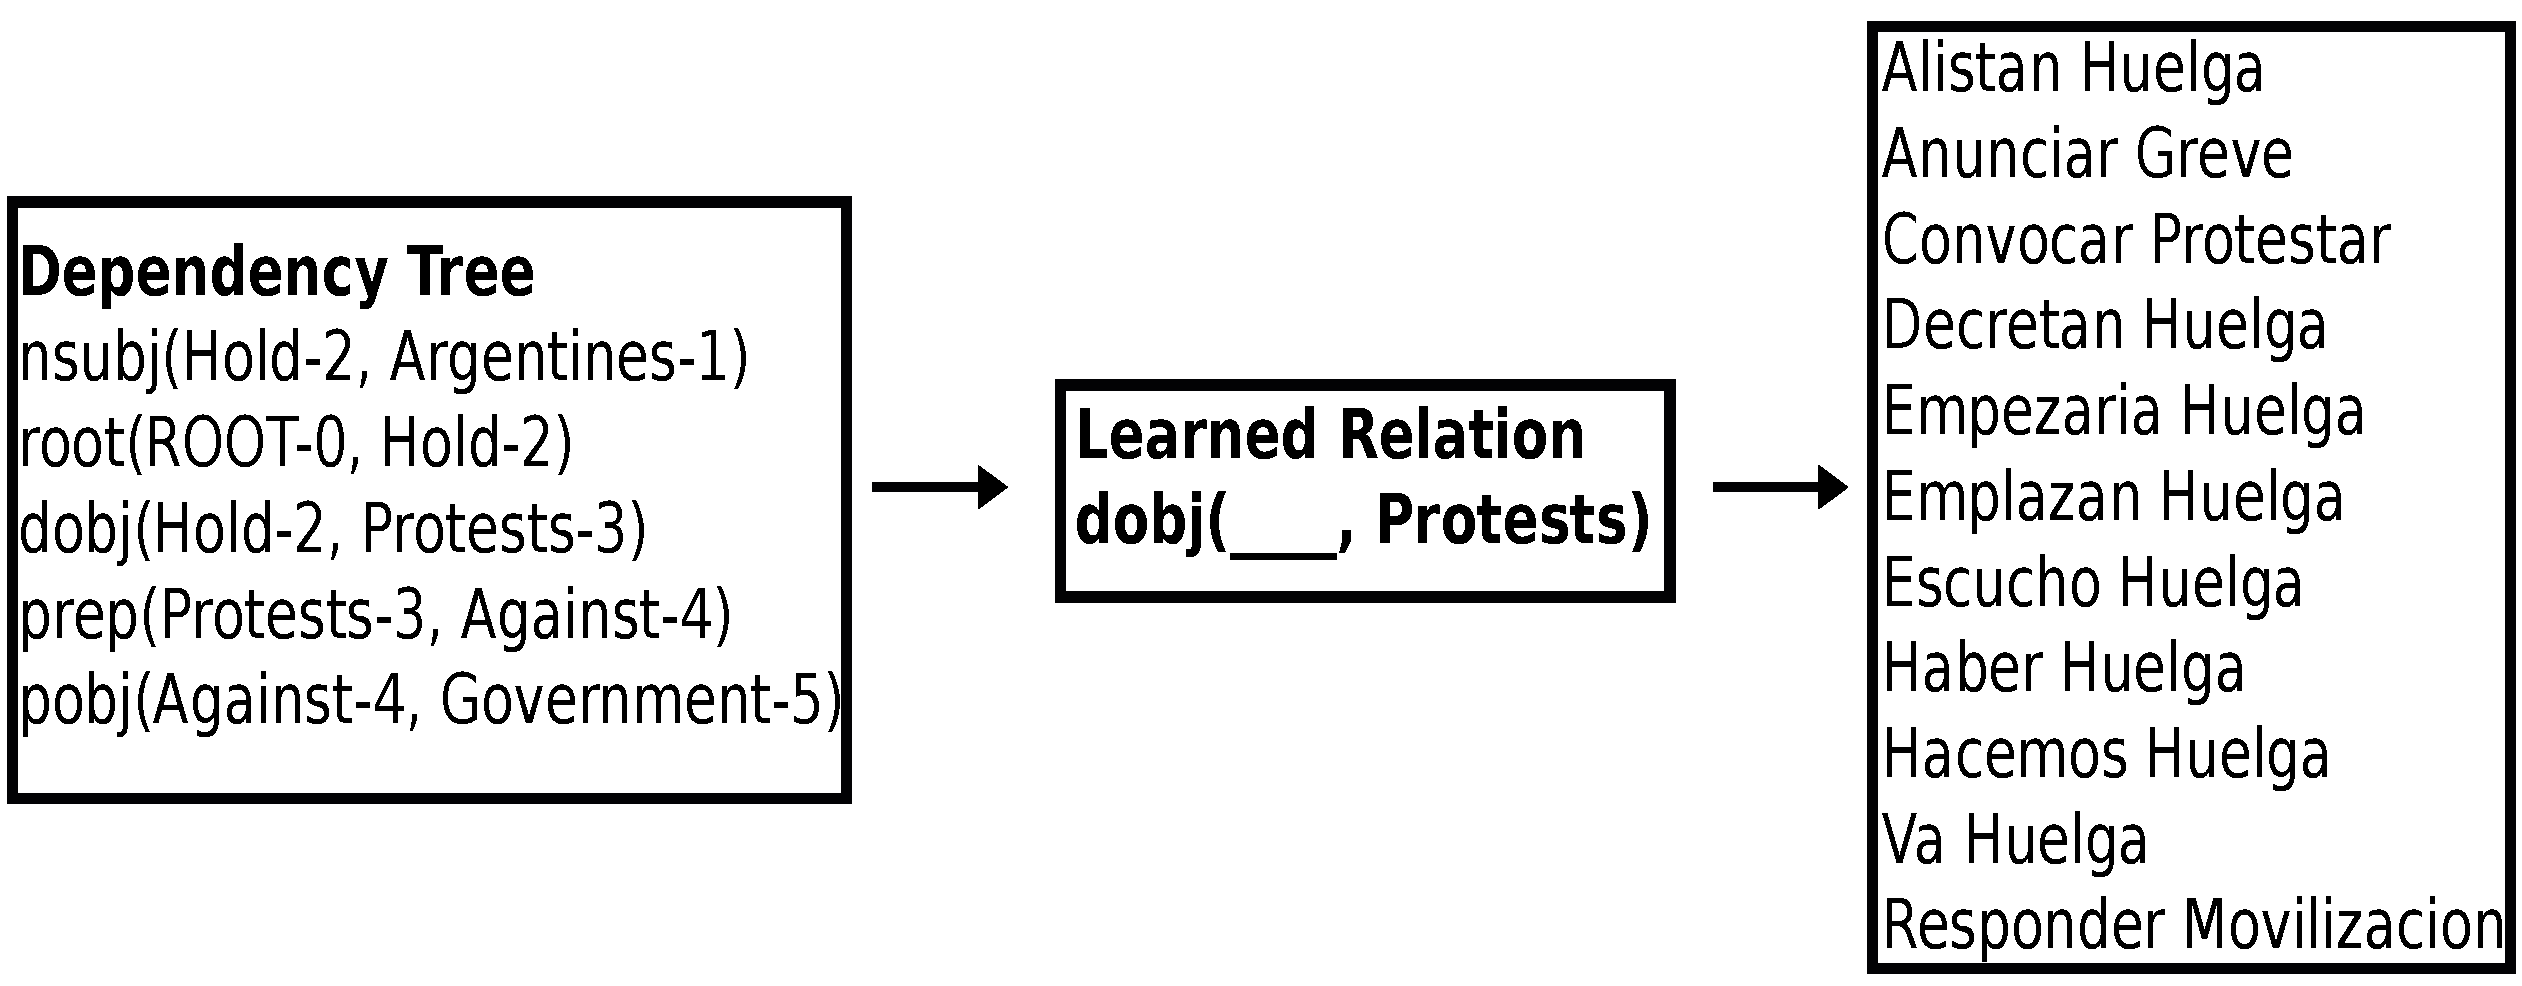
\includegraphics[width=0.5\textwidth]{figures/phraseLearning}
\label{fig:phraselearning}
\end{figure}
